\documentclass[3pt,twocolumn]{elsarticle}
\usepackage[spanish]{babel}
\usepackage[utf8]{inputenc}
\usepackage[hidelinks]{hyperref}
\usepackage{graphics}
\usepackage{graphicx}
\usepackage{epsfig}
\usepackage{amssymb}
\usepackage{amsmath}
\usepackage{amsthm}
\usepackage{lineno}
\usepackage{tikz}
\usepackage{float}
\usepackage{subcaption}
\usepackage{amssymb, amsmath}
\usetikzlibrary{shapes,arrows}
\usepackage{pstricks,pst-node,pst-tree}
%\bibliographystyle{elsarticle-num}

\makeatletter
\renewenvironment{abstract}{\global\setbox\absbox=\vbox\bgroup
\hsize=\textwidth\def\baselinestretch{1}%
\noindent\unskip\textbf{Resumen} 
\par\medskip\noindent\unskip\ignorespaces}
{\egroup}

\def\keyword{%
\def\sep{\unskip, }%
\def\MSC{\@ifnextchar[{\@MSC}{\@MSC[2000]}}
\def\@MSC[##1]{\par\leavevmode\hbox {\it ##1~MSC:\space}}%
\def\PACS{\par\leavevmode\hbox {\it PACS:\space}}%
\def\JEL{\par\leavevmode\hbox {\it JEL:\space}}%
\global\setbox\keybox=\vbox\bgroup\hsize=\textwidth
\normalsize\normalfont\def\baselinestretch{1}
\parskip\z@
\noindent\textit{Palabras clave: } 
\raggedright 
\ignorespaces}

\biboptions{longnamesfirst,comma}

\usepackage{etoolbox}
\makeatletter
\patchcmd{\ps@pprintTitle}% <cmd>
  {Preprint submitted}% <search>
  {Edson\journal{Simulación computacional de nanomateriales.}}% <replace>
  {}{}% <succes><failure>


\makeatother
\begin{document}

\twocolumn[
\begin{@twocolumnfalse}

\begin{frontmatter}
\title{Modelo de análisis térmico en estructuras cristalinas}
\author{Samaniego, E.}
\address{Facultad de Ingeniería Mecánica y Eléctrica, Universidad Autónoma de Nuevo León}

\begin{abstract}
Se realiza un estudio de el comportamiento de las aleaciones de un material puro con cerámicos, polímeros y conductores con el fin de ver que pasa con la conductividad térmica principalmente si llega al punto de fusión dependiendo con que partículas se dope y la manera en que se haga la aleación ya sea distribuida en el material o como una capa superficial para analizar la eficiencia térmica en diferentes grados de temperatura y ver que es preferible, y a su vez ver que ocurre con la conductividad eléctrica del propio material. 
\end{abstract}

\begin{keyword}
Conductividad térmica \sep punto de fusión \sep aleación \sep  
\end{keyword}

\end{frontmatter}
\end{@twocolumnfalse}
]

\section{Introducción}\label{intr}
El estudio de la conductividad térmica en los materiales es de suma importancia para aplicarse en diferentes situaciones para el desarrollo de nuevos materiales para conocer ciertas características de algunas partículas. Las propiedades mecánicas de los materiales pueden controlarse por la adiciones de defecto puntuales como átomos sustitucionales e intersticiales. Particularmente el caso de los metales, los defectos puntuales distorsionan el arreglo atómico en la red, interfiriendo con el movimiento o deslizamiento de las dislocaciones.

La conducción se produce por cesión de energía entre partículas contiguas (vibraciones reticulares) también se debe al movimiento de traslación de los electrones libres \cite{book2}.
La conducción es el único mecanismo de transmisión del calor posible en los medios sólidos. Cuando en estos cuerpos existe un gradiente de temperatura, el calor se transmite de la región de mayor a la de menor temperatura. El flujo real de calor depende de la conductividad térmica, que es una propiedad física del cuerpo. 
Para la integración del estudio térmico en estructuras cristalinas con simulación computacional, es basado en el concepto teórico en que las partículas de un elemento tienen cierta conductividad térmica que puede ser modificada con la adición de otros elementos con menos conductividad térmica para que el material base aumente su resistencia a la temperatura y como afecta su conductividad eléctrica, siendo que a mayor temperatura los átomos superficiales comienzan a vibrar con más intensidad ya que inside más energía en ellos y estas vibraciones se transmiten desde la superficie a el centro del material.

Para generalizar la cantidad de propiedades y cantidades que tiene cada material, en el presente trabajo se realiza una simulación donde se simplifica a porcentajes de conductividad térmica y eléctrica así como valores fijos de tamaño de partículas, para poder analizar como se transmite dicha conductividad, los objetivos de este proyecto son:

\begin{itemize}
    \item Estudiar la conductividad térmica y eléctrica de un material puro y ver su comportamiento gráficamente,
    \item realizar adiciones porcentuales de diferentes materiales para generar simuladamente aleaciones en el material y estudiar su comportamiento de conductividades gráficamente, 
    \item modificar las adiciones a que solo sean superficiales para ver en que afecta a la conductividad tanto eléctrica como térmica,
    \item comparar los distintos resultados y determinar el mejor, siendo que un mejor resultado es tener alto punto de fusión (menor conducción térmica) y buena conducción eléctrica,
    \item para cada resultado estudiar el tiempo en que llega al punto de fusión (si es que llega) variando la temperatura de menos a más en cada caso.
\end{itemize}

\section{Antecedentes}\label{antesc}
Todos aquellos métodos de medida basados en el cambio, con la temperatura o en función del tiempo a temperatura constante, de una propiedad física o mecánica de un material, mientras se le somete a un ambiente de temperaturas controlado, son considerados como análisis térmico \cite{book1}. 
Su importancia y usos más comunes radican en procesos de control de fabricación y en investigaciones.
\subsection{Métodos de medida térmica}
 El objetivo es establecer una relación entre la temperatura y las propiedades físicas del material. El resultado de estas medidas son las curvas de análisis térmico y las características de estas curvas (picos, discontinuidades, cambios de pendiente, etc.) como se muestra en la figura \ref{f1} se relacionan con los eventos térmicos de la muestra.

\begin{figure}[H]
  \centering      
  \includegraphics[scale=.74]{termograma.PNG}
  \caption{Termograma del oxalato cálcico mono hidratado \cite{book1}}
  \label{f1}
\end{figure}
\bigskip

Los equipos termogravimétrico más utilizados son análisis termogravimétrico (TGA). Es una técnica en que la masa de la muestra es controlada contra el tiempo o la temperatura (térmica) mientras que la temperatura de la muestra, en una atmósfera especificada, es programada. Esta técnica ofrece la determinación de composiciones de material. 

En un análisis termogravimétrico se registra, de manera continua, la masa de una muestra colocada en una atmósfera controlada, en función de la temperatura, o bien en función del tiempo. En el primer caso la temperatura de la muestra va aumentando de manera controlada (normalmente de forma lineal con el tiempo) \cite{book1}.

\subsection{Simulación}
Existe actualmente diversos programas para trabajar la simulación que se define como la reproducción (computacional) de fenómenos y procesos del mundo real. Típicamente involucra primero el modelado de dicho proceso o fenómeno a través de experimentos estadísticos \cite{dra}. Las aplicaciones para este método de trabajo son muy diversas ya que puede simularse muchos casos de problemas o métodos graficables cotidianos y las ramas donde se puede utilizar son temas científicos, industriales, de construcción, de la salud, analíticos, finanzas, etc. En el caso para la rama de nanotecnología es posible simular efectos a esta escala (0 a 100 nm) en la que pueden ser mejor representados y los comportamientos se pueden graficar para mejor comprensión ya que estos fenómenos y comportamientos resultan de mucho interés para el estudio y desarrollo de nuevos materiales con propiedades especiales. 

\section{Metodología}
La herramienta principal que se utiliza es el programa \texttt{Python 3.9} \cite{Python}, utilizado para desarrollar la simulación y análisis estadístico de los resultados obtenidos gráficamente.
Este desarrollo de programa es apoyado por librerías como \texttt{Pandas} \cite{pandas} para la creaciones de listas ordenadas donde se almacenan datos que son mas fáciles de llamar y hace el código mas ligero, \texttt{NumPy} \cite{numpy} para sintetizar la manera que se utilizan los arreglos matriciales, vectores de datos,generación de números aleatorios para el caso de las partículas que se grafican y por último \texttt{Matplotlib} \cite{matplot} que es la librería que permite graficar vectores, puntos , diagramas caja-bigote, etc. Esto es de utilidad para la representación e interpretación de datos del código que facilita la comprensión de como se comporta cada material y aleación respecto a las diferentes temperaturas y todo esto dependiendo del porcentaje que se aplica de dopaje al material base, podremos observarlo en diversos gráficos.

\section{Trabajos relacionados}\label{intr}
Para este proyecto hay dos códigos simulados relacionados al comportamiento en el que se basa la simulación tomados como referencia por la similitud en de como se comportan las partículas.
\subsection{Diagramas de Voronoi}
El primer código relacionado es explicado por Schaeffer \cite{DV}, trata de los diagramas de Voronoi donde dichas celdas representan la cristalización de un material con respecto a una cantidad de semillas dadas al azar, posteriormente se estudia el agrietamiento del material y se observa qué tan rápido se distribuye la grieta a través de las uniones de cada semilla y si llega a penetrar el centro del material lo cual ocasionaría una fractura. De manera similar a este código se representa la distribución del calor a través de las partículas y viendo si llega el material al punto de fusión o si nunca llega debido alas propiedades del material o aleaciones agregadas. En lugar de grietas el calor es el que avanza en el material. 

\subsection{Interacciones entre partículas}
Otra práctica similar en demostración computacional es realizada por Schaeffer \cite{IP} que es detallada en su pagina web \cite{dra}, en ella explica y simula interacción entre partículas así como lo son fenómenos de atracción y repulsión en física, cada partícula tiene una carga eléctrica. Cargas de un mismo signo producirán una repulsión mientras cargas opuestas resultan en una atracción la magnitud de la fuerza es proporcional a la diferencia de magnitud de las cargas, y además la fuerza es inversamente proporcional a la distancia euclidiana entre las partículas \cite{IP}. Esto influye en el código de manera que las partículas realizadas tendrán valores dados en porcentajes que impiden o facilitan la conducción de calor o conducción eléctrica, de mismo modo los elementos agregados ya sea polímeros, cerámicos u otros metales tendrán distintas cargas o porcentajes que afectan a la muestra ya sea facilitando o mejorando su conducción.

\section{Solución propuesta }\label{intr}
Para trabajar y encontrar los datos que se tienen de objetivo, es propuesto la idea de representar las partículas de un material base en un plano bidimensional como en la figura \ref{f2}, aunado a esto una partícula (color rojo) que iniciara en la posición \texttt{$(0,0)$} que representa la temperatura como irá adentrándose en el material, para que cada partícula del material base tenga una fuerza que limite el paso de la partícula de calor.

\begin{figure}[H]
  \centering      
  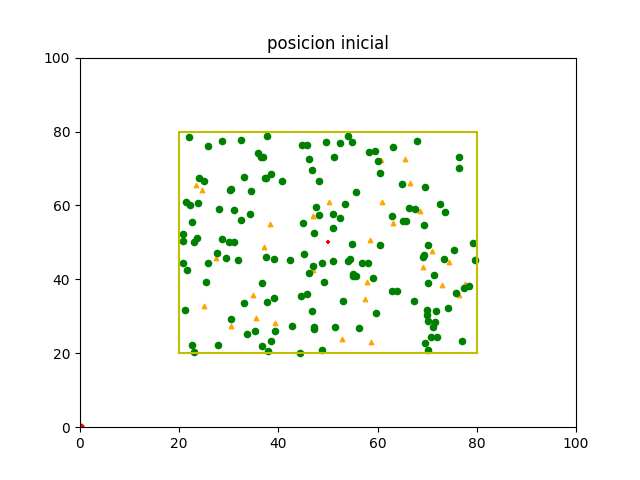
\includegraphics[scale=.5]{p_inicial.png}
  \caption{Plano bidimensional de partículas de material base (puro).}
  \label{f2}
\end{figure}
\bigskip

Como siguiente propuesta para poder recaudar datos de diversos casos según los objetivos, se hace adición para generar aleaciones con partículas cerámicas, polímeros y un material conductor (plata), estas adiciones tienen fuerzas diferentes por partícula (figura \ref{f2} triángulos naranjas) que se interponen al paso de la temperatura según sus propiedades y ésta variación es la que se estudiará. Esta experimentación de las propuestas puede ser visto en el repositorio de Samaniego \cite{Edson} donde se realizaron gif animados por la página GIPHY \cite{GIPHY} para ver el movimiento de la partícula de calor a través del material.

\subsection{Experimentación}
Para la experimentación en base a las propuestas ya se tiene las aleaciones y como la temperatura penetra el material a velocidades distintas según sea el porcentaje de partículas agregadas como dopaje y la otra variante es el valor de la temperatura que en la propuesta es fijo en (45 grados). Entonces lo que se realiza después es automáticamente el cambio de temperaturas para obtener una serie de resultados en el que podamos observar para cada aleación a que temperatura se llega al punto de fusión y en ese punto observar que valor tiene la conductividad eléctrica si tendió a disminuir o aumentar.



\section{Evaluación}\label{intr}
\begin{table}[H]
        \caption{Registro de cada aleación según su porcentaje, distancia máxima al centro(punto de fusión) y tiempo que recorrió.}
        \bigskip
        \label{tab1}
        \centering
        \begin{tabular}{|r|r|r|r|r|r|}
        \hline
         Aleación&Porcentaje&Distancia temperatura&Tiempo&Distancia eléctrica&Tiempo\\
        \hline
         Puro & 25 & 0 & 0 & 0 & 0 \\
        \hline
        Cerámico & 25 & 0 & 0 & 0 & 0 \\
        \hline
         Polímero & 25 & 0 & 0 & 0 & 0\\
        \hline
        Plata & 25 & 0 & 0 & 0 & 0 \\
        \hline
        \end{tabular}
    \end{table}
\section{Conclusiones}\label{intr}

\subsection{Trabajos futuros}

\bibliographystyle{plainnat}
\bibliography{refe}

\end{document}